%%%%
%%%%
%%%%
\chapter{Technological background}
%%%%
%%%%
%%%%

In this chapter I show what technologies are utilized by the framework, to aid its purpose.

\section{Programming languages}


\subsection{XTend}
The framework itself is mostly written in Xtend, which is an extended dialect of Java, with features improving usability, and making it specially useful for implementing code generators. 
Between two \texttt{'''} we can write template expressions.
An example can be seen from the code on \autoref{fig:xtend}, which is a generator for a \cpp{} \texttt{operator==} of a class. 

\begin{figure}[H]
	\begin{center}
		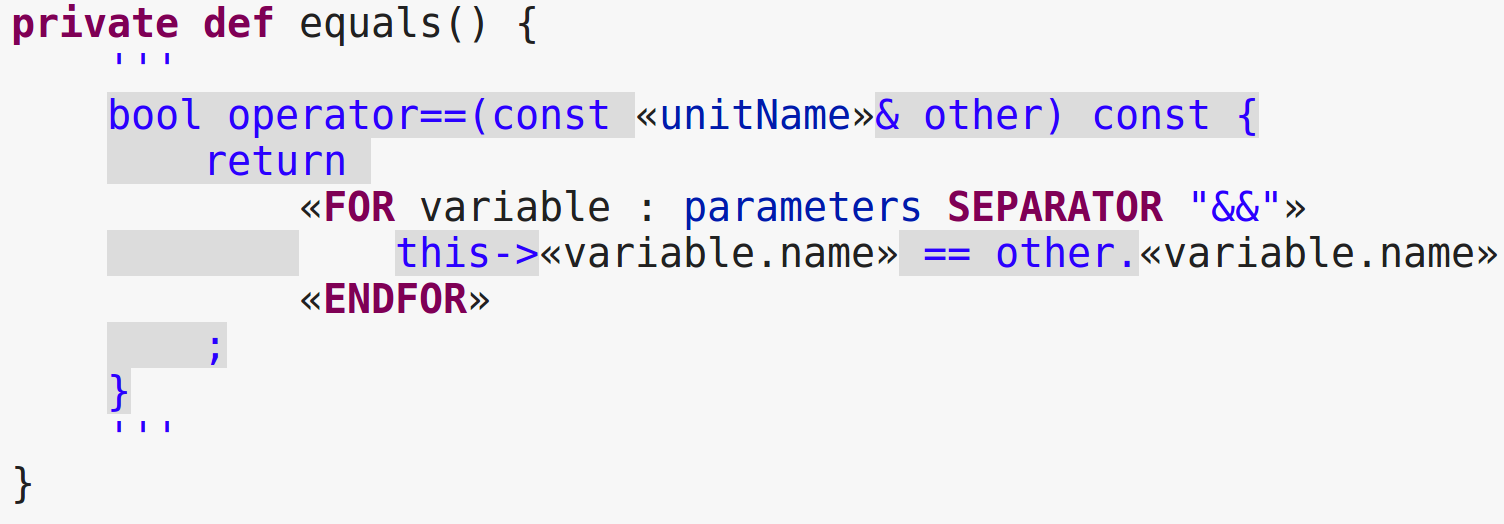
\includegraphics[width=0.8\textwidth]{figures/xtend.png}
		\caption{Template expressions with useful syntax highlight }
		\label{fig:xtend}
	\end{center}
\end{figure}


\subsection{\protect\cpptt }
The generated code is in \cpp{}, because it can be used in various platforms from embedded systems to high powered computers, or virtual machines in clouds. 
Efficiency also considered when choosing \cpp{}, so using embedded systems can be feasible. 

As modern \cpp{} is used in the framework, compiling the code requires a compiler supporting the \cpp{}14 standard.
We use various of modern \cpp{} elements, such as threads, mutexes, lambdas, smart pointers.
Non-generated code also uses templates to handle generated classes, this feature of C++ is extremely useful to integrate the generated code into the framework at compile time.

\section{ Build tools }

To build the generated sources and the \cpp{} libraries we developed, we use Make and CMake utilities. 


Make is a low-level build automaton tool. 
The build is configured by a file called the Makefile.
A Makefile consists of rules. 
A rule has targets (The artifacts generated by the rule), dependencies (artifacts, that must be created to run the rule), and a list of commands, that creates the target artifacts. 
From this declarative configuration file Make can decide the order which commands to run in which order to create a target artifact or multiple target artifacts.
If only some files changes Make only executes the required commands based on timestamps of the files.

As Make is only used in linux systems and larger Makefiles are hard to maintain, we use CMake.
CMake is a higher level tool for build automation. 
It is cross-platform, as CMake configuration files are processed and compiles into project files, like Visual Studio, or Xcode projects, or build scripts for Make or NMake.


\section{Protocol Buffers (Protobuf)}
Protocol Buffers (Protobuf) are a language-neutral, platform-neutral extensible mechanism for serializing structured data \cite{protobuf}. 
We use Protobuf to serialize the data and the messages in query execution.

Protobuf can be used by defining the message structure in \texttt{.proto} files and generating code from them to various languages, which code provide tools for creating, altering, serializing and deserializing messages.

In the framework, message definition for query execution is defined manually, while other messages, that are needed for specific query exeutions are generated by the framework.


\section{DDS -- Data Distibution Service}

DDS~\cite{DDS} is a data exchange standard for real-time systems. 
Its usage is publish-subscribe based.
DDS uses topics which is a relation of corresponding data elements. 
A key specifies the 

We use it to synchronize object and reference creation between computing units of the system.


\section{EMF -- Eclipse Modeling Framework}

Eclipse Modeling Framework is a modeling framework and code generation facility for building tools and other applications based on a structured data model.\cite{emf}.



They are based on Eclipse Modeling Framework (EMF), which provides modeling tools for eclipse based applications.

EMF defines an UML dialect called


\section{\protect\viatra{} }


\viatra{} \cite{viatra} is a framework for model transformations and model querying. 
It provides VQL (Viatra Query Language), a language for graph pattern definition.
\viatra{} can use local search-based and an incremental algorithms to provide matchings for graph patterns. 

In the framework we use the local search planner of \viatra{} and fine tune it to create plans more suitable for our purposes.









